\documentclass[notes,11pt, aspectratio=169]{beamer}

\usepackage{pgfpages}
% These slides also contain speaker notes. You can print just the slides,
% just the notes, or both, depending on the setting below. Comment out the want
% you want.
\setbeameroption{hide notes} % Only slide
%\setbeameroption{show only notes} % Only notes
%\setbeameroption{show notes on second screen=right} % Both

\usepackage{helvet}
\usepackage[default]{lato}
\usepackage{array}
\usepackage{tgbonum}

\usepackage{tikz}
\usepackage{verbatim}
\setbeamertemplate{note page}{\pagecolor{yellow!5}\insertnote}
\usetikzlibrary{positioning}
\usetikzlibrary{calc}
\usetikzlibrary{arrows}
\usetikzlibrary{arrows.meta}
\usetikzlibrary{decorations.markings}
\usetikzlibrary{decorations.pathreplacing}
\usetikzlibrary{shapes.misc}
\usetikzlibrary{shapes.geometric}
\usetikzlibrary{matrix,shapes,arrows,fit,tikzmark}
\usepackage{amsmath}
\usepackage{amssymb}
\usepackage{mathtools}
\usepackage{bm}
\usepackage{mathpazo}
\usepackage{hyperref}
\usepackage{lipsum}
\usepackage{multimedia}
\usepackage{graphicx}
\usepackage{multirow}
\usepackage{dcolumn}
\usepackage{bbm}
\usepackage{pgfplots}
\pgfplotsset{compat=1.18}
\usepackage{listings}
\newcolumntype{d}[0]{D{.}{.}{5}}

\usepackage{changepage}
\usepackage{appendixnumberbeamer}
\newcommand{\beginbackup}{
   \newcounter{framenumbervorappendix}
   \setcounter{framenumbervorappendix}{\value{framenumber}}
   \setbeamertemplate{footline}
   {
     \leavevmode%
     \hline
     box{%
       \begin{beamercolorbox}[wd=\paperwidth,ht=2.25ex,dp=1ex,right]{footlinecolor}%
       \end{beamercolorbox}}%
     \vskip0pt%
   }
 }
\newcommand{\backupend}{
   \addtocounter{framenumbervorappendix}{-\value{framenumber}}
   \addtocounter{framenumber}{\value{framenumbervorappendix}}
}


\usepackage[space]{grffile}
\usepackage{booktabs}
\newcommand\independent{\protect\mathpalette{\protect\independenT}{\perp}}
\def\independenT#1#2{\mathrel{\rlap{$#1#2$}\mkern2mu{#1#2}}}
\DeclareMathOperator{\Supp}{Supp}
\DeclareMathOperator*{\argmin}{arg\,min}

% These are my colors -- there are many like them, but these ones are mine.
\definecolor{blue}{RGB}{0,114,178}
\definecolor{red}{RGB}{213,94,0}
\definecolor{yellow}{RGB}{240,228,66}
\definecolor{green}{RGB}{0,158,115}

\hypersetup{
  colorlinks=true,
  linkbordercolor = {white},
  linkcolor = {blue}
}


%% I use a beige off white for my background
\definecolor{MyBackground}{RGB}{255,253,218}

%% Uncomment this if you want to change the background color to something else
%\setbeamercolor{background canvas}{bg=MyBackground}

%% Change the bg color to adjust your transition slide background color!
\newenvironment{transitionframe}{
  \setbeamercolor{background canvas}{bg=yellow}
  \begin{frame}}{
    \end{frame}
}

\setbeamercolor{frametitle}{fg=blue}
\setbeamercolor{title}{fg=black}
\setbeamertemplate{footline}[frame number]
\setbeamertemplate{navigation symbols}{}
\setbeamertemplate{itemize items}{-}
\setbeamercolor{itemize item}{fg=blue}
\setbeamercolor{itemize subitem}{fg=blue}
\setbeamercolor{enumerate item}{fg=blue}
\setbeamercolor{enumerate subitem}{fg=blue}
\setbeamercolor{button}{bg=MyBackground,fg=blue,}

\setbeamercolor{section in toc}{fg=blue}
\setbeamercolor{subsection in toc}{fg=red}
\setbeamersize{text margin left=1em,text margin right=1em}

\newenvironment{wideitemize}{\itemize\addtolength{\itemsep}{10pt}}{\enditemize}

\usepackage{environ}

% ---- Code listing style ----
\lstset{
    language=Python,
    basicstyle=\ttfamily\scriptsize,
    keywordstyle=\color{blue}\bfseries,
    stringstyle=\color{red!70!black},
    commentstyle=\color{green!50!black}\itshape,
    numbers=left,
    numberstyle=\tiny\color{gray},
    numbersep=5pt,
    frame=single,
    breaklines=true,
    backgroundcolor=\color{gray!5},
    showstringspaces=false,
    tabsize=4
}

% ---- Math shortcuts ----
\newcommand{\vx}{\mathbf{x}}
\newcommand{\vw}{\mathbf{w}}
\newcommand{\vb}{\mathbf{b}}
\newcommand{\vh}{\mathbf{h}}
\newcommand{\vy}{\mathbf{y}}
\newcommand{\vz}{\mathbf{z}}
\newcommand{\vW}{\mathbf{W}}
\newcommand{\R}{\mathbb{R}}
\newcommand{\E}{\mathbb{E}}


\title[]{\textcolor{blue}{Advanced Methods in Deep Learning}\\ \textcolor{black}{\normalsize Lecture 1: Introduction to Deep Learning and Perceptrons}}
\author[Quispe]{}
\institute[MECA]{\small{Alexander Quispe Rojas \\ Universidad del Pac\'ifico -- MECA  \\ aw.quispero@up.edu.pe \quad aquisper@caltech.edu}}
\date{April 13, 2026}


\begin{document}

%%% TIKZ STUFF
\tikzset{
        every picture/.style={remember picture,baseline},
        every node/.style={anchor=base,align=center,outer sep=1.5pt},
        every path/.style={thick},
        }
\newcommand\marktopleft[1]{%
    \tikz[overlay,remember picture]
        \node (marker-#1-a) at (-.3em,.3em) {};%
}
\newcommand\markbottomright[2]{%
    \tikz[overlay,remember picture]
        \node (marker-#1-b) at (0em,0em) {};%
}
\tikzstyle{every picture}+=[remember picture]
\tikzstyle{mybox} =[draw=black, very thick, rectangle, inner sep=10pt, inner ysep=20pt]
\tikzstyle{fancytitle} =[draw=black,fill=red, text=white]
%%%% END TIKZ STUFF

% ============================================================
% Title Slide
% ============================================================
\begin{frame}
\maketitle
\end{frame}

% ============================================================
% Roadmap
% ============================================================
\begin{frame}
\frametitle{Today's Roadmap}
\tableofcontents
\end{frame}


% ============================================================
\section{Course Overview and Motivation}
% ============================================================

\begin{transitionframe}
\begin{center}
{\Huge \textbf{Course Overview \& Motivation}}
\end{center}
\end{transitionframe}

% ---- What is Deep Learning ----
\begin{frame}
\frametitle{What is Deep Learning?}

\begin{columns}[T]
\begin{column}{0.55\textwidth}
\textbf{Machine Learning:} algorithms that learn from data.

\vspace{6pt}
\textbf{Deep Learning:} a subset of ML that uses \textcolor{red}{neural networks with multiple layers} to learn hierarchical representations of data.

\vspace{6pt}
\textbf{Key idea:}
\begin{wideitemize}
    \item Instead of hand-engineering features, the model \emph{learns} the right representation.
    \item Each layer transforms the data into a more useful representation.
    \item \textbf{Depth} = number of stages of processing.
\end{wideitemize}
\end{column}

\begin{column}{0.42\textwidth}
\begin{center}
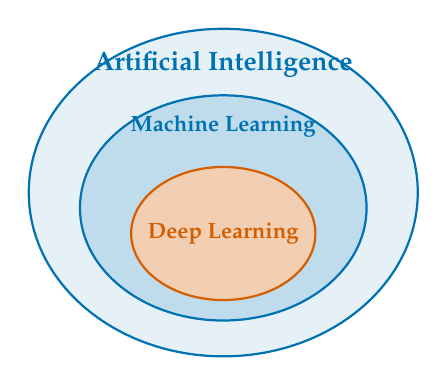
\begin{tikzpicture}[scale=0.65, every node/.style={scale=0.8}]
    \draw[fill=blue!10, draw=blue, thick] (0,0) ellipse (3.8cm and 3.2cm);
    \node[blue, font=\large\bfseries] at (0, 2.5) {Artificial Intelligence};

    \draw[fill=blue!25, draw=blue, thick] (0,-0.3) ellipse (2.8cm and 2.2cm);
    \node[blue, font=\bfseries] at (0, 1.3) {Machine Learning};

    \draw[fill=red!30, draw=red, thick] (0,-0.8) ellipse (1.8cm and 1.3cm);
    \node[red, font=\bfseries] at (0, -0.8) {Deep Learning};
\end{tikzpicture}
\end{center}
\end{column}
\end{columns}
\end{frame}

% ---- Why Now ----
\begin{frame}
\frametitle{Why Deep Learning Now?}

Three ingredients came together:

\vspace{6pt}
\begin{columns}[T]
\begin{column}{0.32\textwidth}
\centering
\textcolor{blue}{\textbf{1. Data}}\\[6pt]
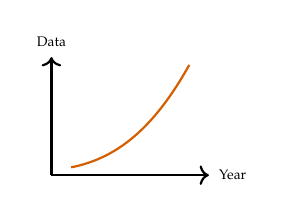
\begin{tikzpicture}[scale=0.5]
    \draw[thick, ->] (0,0) -- (4,0) node[right] {\tiny Year};
    \draw[thick, ->] (0,0) -- (0,3) node[above] {\tiny Data};
    \draw[thick, red] (0.5, 0.2) .. controls (1.5, 0.4) and (2.5, 1.0) .. (3.5, 2.8);
\end{tikzpicture}
\\[4pt]
{\small Internet, digitization, sensors, satellites}
\end{column}

\begin{column}{0.32\textwidth}
\centering
\textcolor{blue}{\textbf{2. Compute (GPUs)}}\\[6pt]
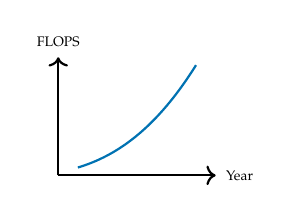
\begin{tikzpicture}[scale=0.5]
    \draw[thick, ->] (0,0) -- (4,0) node[right] {\tiny Year};
    \draw[thick, ->] (0,0) -- (0,3) node[above] {\tiny FLOPS};
    \draw[thick, blue] (0.5, 0.2) .. controls (1.5, 0.5) and (2.5, 1.2) .. (3.5, 2.8);
\end{tikzpicture}
\\[4pt]
{\small NVIDIA GPUs, Google TPUs, cloud computing}
\end{column}

\begin{column}{0.32\textwidth}
\centering
\textcolor{blue}{\textbf{3. Algorithms}}\\[6pt]
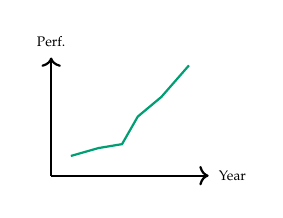
\begin{tikzpicture}[scale=0.5]
    \draw[thick, ->] (0,0) -- (4,0) node[right] {\tiny Year};
    \draw[thick, ->] (0,0) -- (0,3) node[above] {\tiny Perf.};
    \draw[thick, green] (0.5, 0.5) -- (1.2, 0.7) -- (1.8, 0.8) -- (2.2, 1.5) -- (2.8, 2.0) -- (3.5, 2.8);
\end{tikzpicture}
\\[4pt]
{\small Backpropagation, ReLU, dropout, Transformers}
\end{column}
\end{columns}

\vspace{10pt}
\begin{center}
\textcolor{red}{Neural networks existed since the 1950s --- what changed is the scale.}
\end{center}
\end{frame}

% ---- Brief History ----
\begin{frame}
\frametitle{A Brief History of Neural Networks}
\begin{center}
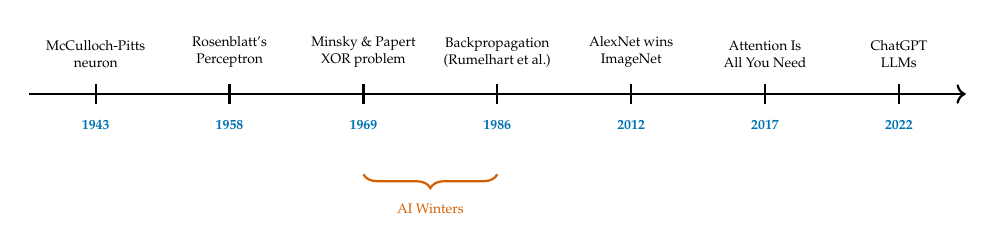
\begin{tikzpicture}[scale=0.85]
    \draw[thick, ->] (0,0) -- (14,0);

    % 1943
    \draw[thick] (1, -0.15) -- (1, 0.15);
    \node[below, font=\tiny\bfseries, text=blue] at (1, -0.25) {1943};
    \node[above, align=center, font=\tiny] at (1, 0.25) {McCulloch-Pitts\\neuron};
    % 1958
    \draw[thick] (3, -0.15) -- (3, 0.15);
    \node[below, font=\tiny\bfseries, text=blue] at (3, -0.25) {1958};
    \node[above, align=center, font=\tiny] at (3, 0.25) {Rosenblatt's\\Perceptron};
    % 1969
    \draw[thick] (5, -0.15) -- (5, 0.15);
    \node[below, font=\tiny\bfseries, text=blue] at (5, -0.25) {1969};
    \node[above, align=center, font=\tiny] at (5, 0.25) {Minsky \& Papert\\XOR problem};
    % 1986
    \draw[thick] (7, -0.15) -- (7, 0.15);
    \node[below, font=\tiny\bfseries, text=blue] at (7, -0.25) {1986};
    \node[above, align=center, font=\tiny] at (7, 0.25) {Backpropagation\\(Rumelhart et al.)};
    % 2012
    \draw[thick] (9, -0.15) -- (9, 0.15);
    \node[below, font=\tiny\bfseries, text=blue] at (9, -0.25) {2012};
    \node[above, align=center, font=\tiny] at (9, 0.25) {AlexNet wins\\ImageNet};
    % 2017
    \draw[thick] (11, -0.15) -- (11, 0.15);
    \node[below, font=\tiny\bfseries, text=blue] at (11, -0.25) {2017};
    \node[above, align=center, font=\tiny] at (11, 0.25) {Attention Is\\All You Need};
    % 2022
    \draw[thick] (13, -0.15) -- (13, 0.15);
    \node[below, font=\tiny\bfseries, text=blue] at (13, -0.25) {2022};
    \node[above, align=center, font=\tiny] at (13, 0.25) {ChatGPT\\LLMs};

    \draw[decorate, decoration={brace, amplitude=5pt, mirror}, thick, red] (5, -1.2) -- (7, -1.2);
    \node[below, text=red, font=\tiny] at (6, -1.5) {AI Winters};
\end{tikzpicture}
\end{center}

\vspace{4pt}
\begin{wideitemize}
    \item \textbf{1943--1969:} Early excitement $\to$ crushed by XOR limitation.
    \item \textbf{1986:} Backpropagation revives interest, but limited by compute.
    \item \textbf{2012:} Deep CNNs dominate computer vision (AlexNet).
    \item \textbf{2017--now:} Transformers $\to$ LLMs $\to$ foundation models revolution.
\end{wideitemize}
\end{frame}

% ---- DL in Economics ----
\begin{frame}
\frametitle{Deep Learning in Economics -- Why Should You Care?}

\begin{columns}[T]
\begin{column}{0.48\textwidth}
\textcolor{blue}{\textbf{Text as Data}}
\begin{itemize}
    \item Sentiment analysis of central bank minutes.
    \item Classification of policy documents.
    \item NLP on congressional speeches.
\end{itemize}
{\tiny Hansen \& McMahon (2016), Gentzkow et al.\ (2019)}

\vspace{8pt}
\textcolor{blue}{\textbf{Satellite Imagery}}
\begin{itemize}
    \item Predicting poverty from nightlight data.
    \item Measuring economic activity.
    \item Agricultural output estimation.
\end{itemize}
{\tiny Jean et al.\ (2016, \emph{Science})}
\end{column}

\begin{column}{0.48\textwidth}
\textcolor{blue}{\textbf{Prediction \& Forecasting}}
\begin{itemize}
    \item GDP nowcasting with unstructured data.
    \item Financial market prediction.
    \item Consumer behavior modeling.
\end{itemize}
{\tiny Athey \& Imbens (2019)}

\vspace{8pt}
\textcolor{blue}{\textbf{Causal Inference + DL}}
\begin{itemize}
    \item Double/debiased ML with neural nets.
    \item Heterogeneous treatment effects.
    \item Instrumental variables with DL.
\end{itemize}
{\tiny Chernozhukov et al.\ (2018)}
\end{column}
\end{columns}
\end{frame}

% ---- Course Roadmap ----
\begin{frame}
\frametitle{Course Roadmap}
\begin{center}
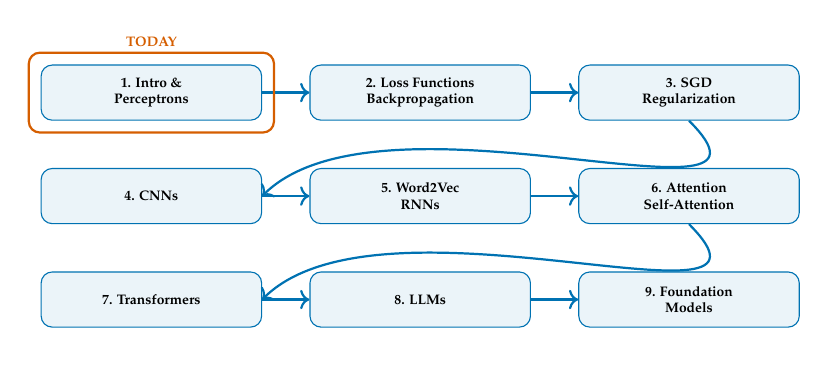
\begin{tikzpicture}[
    node distance=0.4cm and 0.6cm,
    block/.style={rectangle, draw=blue, fill=blue!8, rounded corners,
                  minimum height=0.7cm, minimum width=2.8cm, align=center, font=\tiny\bfseries},
    arrow/.style={->, thick, blue}
]
    \node[block] (s1) {1. Intro \&\\Perceptrons};
    \node[block, right=of s1] (s2) {2. Loss Functions\\Backpropagation};
    \node[block, right=of s2] (s3) {3. SGD\\Regularization};

    \node[block, below=0.6cm of s1] (s4) {4. CNNs};
    \node[block, right=of s4] (s5) {5. Word2Vec\\RNNs};
    \node[block, right=of s5] (s6) {6. Attention\\Self-Attention};

    \node[block, below=0.6cm of s4] (s7) {7. Transformers};
    \node[block, right=of s7] (s8) {8. LLMs};
    \node[block, right=of s8] (s9) {9. Foundation\\Models};

    \draw[arrow] (s1) -- (s2);
    \draw[arrow] (s2) -- (s3);
    \draw[arrow] (s3.south) to[out=-45, in=45] (s4.east);
    \draw[arrow] (s4) -- (s5);
    \draw[arrow] (s5) -- (s6);
    \draw[arrow] (s6.south) to[out=-45, in=45] (s7.east);
    \draw[arrow] (s7) -- (s8);
    \draw[arrow] (s8) -- (s9);

    \draw[thick, red, rounded corners] ([shift={(-0.15,-0.15)}]s1.south west) rectangle ([shift={(0.15,0.15)}]s1.north east);
    \node[red, font=\tiny\bfseries, above=0.1cm of s1] {TODAY};
\end{tikzpicture}
\end{center}

\vspace{4pt}
\textbf{Evaluation:} 4 Homeworks (60\%) + Oral Exam (30\%) + Participation (10\%)

\textbf{Tools:} Python, PyTorch, Google Colab \quad | \quad LLMs encouraged (Claude Code, ChatGPT)
\end{frame}


% ============================================================
\section{The Supervised Learning Problem}
% ============================================================

\begin{transitionframe}
\begin{center}
{\Huge \textbf{The Supervised Learning Problem}}
\end{center}
\end{transitionframe}

% ---- Supervised Learning Setup ----
\begin{frame}
\frametitle{Supervised Learning: The Setup}

\begin{tikzpicture}
\node [mybox] (box){%
    \begin{minipage}{0.93\textwidth}
    \textbf{Given:}
    \begin{itemize}
        \item A dataset of $N$ input-output pairs: $\mathcal{D} = \{(\vx_1, y_1), (\vx_2, y_2), \ldots, (\vx_N, y_N)\}$.
        \item Each input: $\vx_i \in \R^d$ \quad (a vector of $d$ features).
        \item Each output: $y_i \in \mathcal{Y}$ \quad (the target/label).
    \end{itemize}

    \vspace{6pt}
    \textbf{Goal:} Find a function $f: \R^d \to \mathcal{Y}$ that maps inputs to outputs, such that $f$ \textcolor{red}{generalizes} well to \textbf{unseen data}.
    \end{minipage}
};
\node[fancytitle, right=10pt] at (box.north west) {The Learning Problem};
\end{tikzpicture}

\vspace{10pt}
\textbf{Two types of problems:}
\begin{columns}[T]
\begin{column}{0.45\textwidth}
\centering
\textcolor{blue}{\textbf{Regression:}} $y \in \R$ (continuous)\\
{\small e.g., predict GDP growth, house prices.}
\end{column}
\begin{column}{0.45\textwidth}
\centering
\textcolor{blue}{\textbf{Classification:}} $y \in \{0, 1, \ldots, K\}$ (discrete)\\
{\small e.g., spam detection, recession indicator.}
\end{column}
\end{columns}
\end{frame}

% ---- Regression vs Classification ----
\begin{frame}
\frametitle{Regression vs.\ Classification}

\begin{columns}
\begin{column}{0.48\textwidth}
\centering
\textcolor{blue}{\textbf{Regression:}} $y$ is continuous

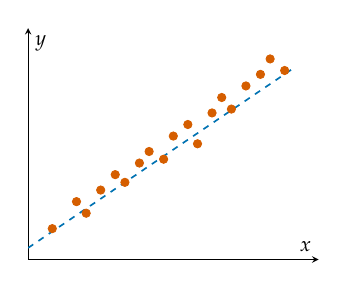
\begin{tikzpicture}[scale=0.75]
    \begin{axis}[
        xlabel={$x$}, ylabel={$y$},
        xmin=0, xmax=6, ymin=0, ymax=6,
        width=6.5cm, height=5.5cm,
        axis lines=middle,
        ticks=none
    ]
    \addplot[only marks, mark=*, mark size=2pt, red] coordinates {
        (0.5,0.8) (1,1.5) (1.2,1.2) (1.5,1.8) (1.8,2.2) (2,2.0)
        (2.3,2.5) (2.5,2.8) (2.8,2.6) (3,3.2) (3.3,3.5) (3.5,3.0)
        (3.8,3.8) (4,4.2) (4.2,3.9) (4.5,4.5) (4.8,4.8) (5,5.2)
        (5.3,4.9)
    };
    \addplot[thick, blue, dashed, domain=0:5.5] {0.85*x + 0.3};
    \end{axis}
\end{tikzpicture}

{\small $f(\vx) = \vw^\top \vx + b$}
\end{column}

\begin{column}{0.48\textwidth}
\centering
\textcolor{blue}{\textbf{Classification:}} $y$ is binary/categorical

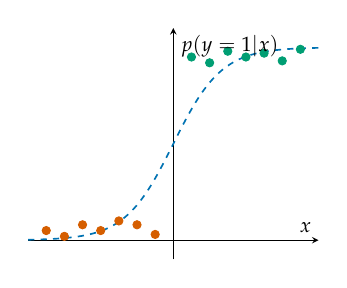
\begin{tikzpicture}[scale=0.75]
    \begin{axis}[
        xlabel={$x$}, ylabel={$p(y=1|x)$},
        xmin=-4, xmax=4, ymin=-0.1, ymax=1.1,
        width=6.5cm, height=5.5cm,
        axis lines=middle,
        ticks=none
    ]
    \addplot[thick, blue, dashed, domain=-4:4, samples=100] {1/(1+exp(-1.5*x))};
    \addplot[only marks, mark=*, mark size=2pt, red] coordinates {
        (-3.5,0.05) (-3,0.02) (-2.5,0.08) (-2,0.05) (-1.5,0.1) (-1,0.08) (-0.5,0.03)
    };
    \addplot[only marks, mark=*, mark size=2pt, green] coordinates {
        (0.5,0.95) (1,0.92) (1.5,0.98) (2,0.95) (2.5,0.97) (3,0.93) (3.5,0.99)
    };
    \end{axis}
\end{tikzpicture}

{\small $p(y=1|\vx) = \sigma(\vw^\top \vx + b)$}
\end{column}
\end{columns}

\vspace{8pt}
\begin{center}
\textcolor{red}{In both cases: we choose a \textbf{model}, define a \textbf{loss}, and \textbf{optimize}.}
\end{center}
\end{frame}

% ---- Connection to Econometrics ----
\begin{frame}
\frametitle{Connection to Econometrics}

\begin{tikzpicture}
\node [mybox] (box){%
    \begin{minipage}{0.93\textwidth}
    \textbf{OLS regression} is a special case of supervised learning:
    \[
        y_i = \beta_0 + \beta_1 x_{i1} + \beta_2 x_{i2} + \cdots + \beta_d x_{id} + \varepsilon_i
    \]
    \begin{itemize}
        \item Model: $f(\vx) = \vw^\top \vx + b$ \quad (linear hypothesis).
        \item Loss: $\mathcal{L} = \frac{1}{N}\sum_{i=1}^{N}(y_i - f(\vx_i))^2$ \quad (MSE = OLS objective).
        \item Optimization: closed-form solution $\hat{\bm{\beta}} = (\mathbf{X}^\top\mathbf{X})^{-1}\mathbf{X}^\top\vy$.
    \end{itemize}
    \end{minipage}
};
\node[fancytitle, right=10pt] at (box.north west) {What you already know};
\end{tikzpicture}

\vspace{6pt}
\textbf{What deep learning adds:}
\begin{wideitemize}
    \item Replace the \textbf{linear model} with a \textcolor{red}{non-linear, multi-layer} function.
    \item Replace the \textbf{closed-form solution} with \textcolor{red}{iterative optimization} (gradient descent).
    \item Replace \textbf{hand-crafted features} with \textcolor{red}{learned representations}.
    \item Trade-off: \textbf{interpretability} $\leftrightarrow$ \textbf{predictive power}.
\end{wideitemize}
\end{frame}

% ---- Hypothesis Set ----
\begin{frame}
\frametitle{The Hypothesis Set}

\begin{tikzpicture}
\node [mybox] (box){%
    \begin{minipage}{0.93\textwidth}
    A \textbf{hypothesis set} $\mathcal{H}$ is the space of candidate functions the learning algorithm can choose from to map inputs $\vx$ to outputs $y$.
    \end{minipage}
};
\node[fancytitle, right=10pt] at (box.north west) {Definition};
\end{tikzpicture}

\vspace{8pt}
\textbf{Examples:}

\renewcommand{\arraystretch}{1.5}
\begin{center}
\begin{tabular}{lll}
\toprule
\textbf{Model} & \textbf{Hypothesis set $\mathcal{H}$} & \textbf{Complexity} \\
\midrule
Linear regression & $\{f(\vx) = \vw^\top \vx + b : \vw \in \R^d, b \in \R\}$ & Low \\
Polynomial & $\{f(\vx) = \sum_{|\alpha| \leq p} w_\alpha \vx^\alpha\}$ & Medium \\
Neural network & $\{f(\vx) = \vW^{(L)}\sigma(\cdots\sigma(\vW^{(1)}\vx + \vb^{(1)})\cdots) + \vb^{(L)}\}$ & \textcolor{red}{High} \\
\bottomrule
\end{tabular}
\end{center}

\vspace{10pt}
\begin{center}
\textcolor{red}{Deep learning = very rich hypothesis set + data-driven optimization.}
\end{center}
\end{frame}

% ---- Training vs Test ----
\begin{frame}
\frametitle{Training Data vs.\ Test Data}

\begin{columns}[T]
\begin{column}{0.55\textwidth}
\textcolor{blue}{\textbf{Training set}} $\mathcal{D}_{\text{train}}$:
\begin{itemize}
    \item Used to learn the model parameters.
    \item We observe both $\vx$ and $y$.
\end{itemize}

\vspace{6pt}
\textcolor{blue}{\textbf{Test set}} $\mathcal{D}_{\text{test}}$:
\begin{itemize}
    \item Used \emph{only} to evaluate generalization.
    \item \textcolor{red}{Never} use test data to modify the model.
\end{itemize}

\vspace{6pt}
\textcolor{blue}{\textbf{Validation set}} $\mathcal{D}_{\text{val}}$:
\begin{itemize}
    \item Used to tune hyperparameters.
    \item Select model complexity.
\end{itemize}

\vspace{6pt}
\textbf{Key Principle:} The goal is \textcolor{red}{generalization} --- performing well on data the model has \emph{never seen}.
\end{column}

\begin{column}{0.42\textwidth}
\begin{center}
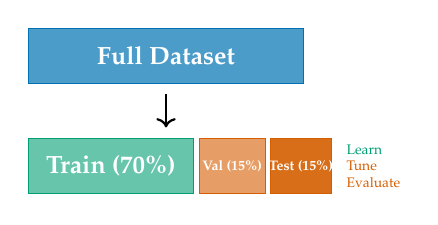
\begin{tikzpicture}[scale=0.7]
    \draw[fill=blue!70, draw=blue] (0,0) rectangle (5,1);
    \node[white, font=\small\bfseries] at (2.5, 0.5) {Full Dataset};

    \draw[->, thick] (2.5, -0.2) -- (2.5, -0.8);

    \draw[fill=green!60, draw=green] (0,-1) rectangle (3,-2);
    \node[white, font=\small\bfseries] at (1.5, -1.5) {Train (70\%)};

    \draw[fill=red!60, draw=red] (3.1,-1) rectangle (4.3,-2);
    \node[white, font=\tiny\bfseries] at (3.7, -1.5) {Val (15\%)};

    \draw[fill=red!90, draw=red] (4.4,-1) rectangle (5.5,-2);
    \node[white, font=\tiny\bfseries] at (4.95, -1.5) {Test (15\%)};

    \node[green, font=\tiny, right] at (5.6, -1.2) {Learn};
    \node[red, font=\tiny, right] at (5.6, -1.5) {Tune};
    \node[red, font=\tiny, right] at (5.6, -1.8) {Evaluate};
\end{tikzpicture}
\end{center}
\end{column}
\end{columns}
\end{frame}

% ---- Overfitting ----
\begin{frame}
\frametitle{Overfitting vs.\ Underfitting}

\begin{center}
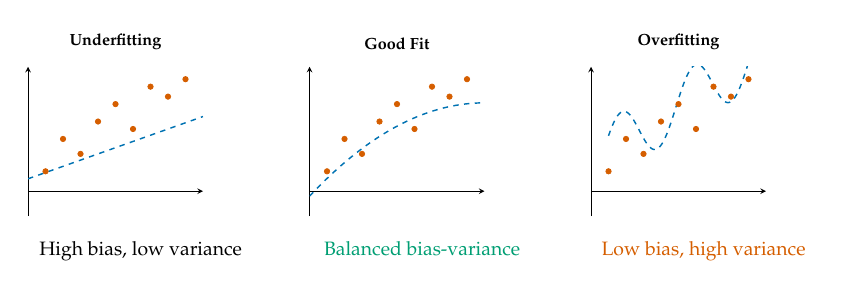
\begin{tikzpicture}[scale=0.65]
    \begin{scope}[shift={(0,0)}]
        \begin{axis}[
            title={\small\textbf{Underfitting}},
            width=5cm, height=4.5cm,
            xmin=0, xmax=5, ymin=-1, ymax=5,
            axis lines=middle, ticks=none
        ]
        \addplot[only marks, mark=*, mark size=1.5pt, red] coordinates {
            (0.5,0.8) (1,2.1) (1.5,1.5) (2,2.8) (2.5,3.5) (3,2.5)
            (3.5,4.2) (4,3.8) (4.5,4.5)
        };
        \addplot[thick, blue, dashed, domain=0:5] {0.5*x + 0.5};
        \end{axis}
        \node[below, font=\scriptsize] at (2.2, -0.3) {High bias, low variance};
    \end{scope}

    \begin{scope}[shift={(5.5,0)}]
        \begin{axis}[
            title={\small\textbf{Good Fit}},
            width=5cm, height=4.5cm,
            xmin=0, xmax=5, ymin=-1, ymax=5,
            axis lines=middle, ticks=none
        ]
        \addplot[only marks, mark=*, mark size=1.5pt, red] coordinates {
            (0.5,0.8) (1,2.1) (1.5,1.5) (2,2.8) (2.5,3.5) (3,2.5)
            (3.5,4.2) (4,3.8) (4.5,4.5)
        };
        \addplot[thick, blue, dashed, domain=0:5, samples=50] {-0.15*x^2 + 1.5*x - 0.2};
        \end{axis}
        \node[below, font=\scriptsize, text=green] at (2.2, -0.3) {Balanced bias-variance};
    \end{scope}

    \begin{scope}[shift={(11,0)}]
        \begin{axis}[
            title={\small\textbf{Overfitting}},
            width=5cm, height=4.5cm,
            xmin=0, xmax=5, ymin=-1, ymax=5,
            axis lines=middle, ticks=none
        ]
        \addplot[only marks, mark=*, mark size=1.5pt, red] coordinates {
            (0.5,0.8) (1,2.1) (1.5,1.5) (2,2.8) (2.5,3.5) (3,2.5)
            (3.5,4.2) (4,3.8) (4.5,4.5)
        };
        % Wiggly curve that passes close to every point
        \addplot[thick, blue, dashed, samples=200, domain=0.5:4.5]
            {1.2 + 0.9*x + 1.2*sin(deg(3*x - 1))};
        \end{axis}
        \node[below, font=\scriptsize, text=red] at (2.2, -0.3) {Low bias, high variance};
    \end{scope}
\end{tikzpicture}
\end{center}

\vspace{4pt}
\textbf{Overfitting:} the model memorizes training data (including noise) and fails to generalize.

\textbf{Prevention:} regularization (L1, L2), early stopping, dropout, more data.

\vspace{4pt}
\begin{center}
\textcolor{red}{Deep networks have millions of parameters --- overfitting is a central concern.}
\end{center}
\end{frame}


% ============================================================
\section{Linear Models as Starting Point}
% ============================================================

\begin{transitionframe}
\begin{center}
{\Huge \textbf{Linear Models: The Starting Point}}
\end{center}
\end{transitionframe}

% ---- Linear Regression ----
\begin{frame}
\frametitle{Linear Regression}

\begin{tikzpicture}
\node [mybox] (box){%
    \begin{minipage}{0.93\textwidth}
    \[
        f(\vx) = \vw^\top \vx + b = w_1 x_1 + w_2 x_2 + \cdots + w_d x_d + b
    \]
    where $\vw \in \R^d$ is the \textbf{weight vector} and $b \in \R$ is the \textbf{bias}.
    \end{minipage}
};
\node[fancytitle, right=10pt] at (box.north west) {Model};
\end{tikzpicture}

\vspace{6pt}
\textbf{Loss function:} Mean Squared Error (MSE)
\[
    \mathcal{L}(\vw, b) = \frac{1}{N}\sum_{i=1}^{N}\left(y_i - f(\vx_i)\right)^2 = \frac{1}{N}\sum_{i=1}^{N}\left(y_i - \vw^\top \vx_i - b\right)^2
\]

\vspace{6pt}
\textbf{Goal:} Find the parameters $(\vw^*, b^*)$ that minimize the loss:
\[
    \vw^*, b^* = \argmin_{\vw, b} \; \mathcal{L}(\vw, b)
\]

\vspace{4pt}
\textbf{Closed-form solution} (via $\nabla_{\vw}\mathcal{L} = 0$): \quad $\hat{\vw} = (\mathbf{X}^\top\mathbf{X})^{-1}\mathbf{X}^\top\vy$.

\vspace{4pt}
{\small \textit{This is exactly OLS --- the starting point for all of deep learning.}}
\end{frame}

% ---- Logistic Regression ----
\begin{frame}
\frametitle{Logistic Regression for Classification}

For \textbf{binary classification} ($y \in \{0, 1\}$), we need $f(\vx) \in [0,1]$.

\vspace{4pt}
\textbf{Step 1:} Apply the \textbf{sigmoid function} $\sigma$ to the linear model:
\[
    p(y = 1 | \vx) = \sigma(\vw^\top \vx + b) = \frac{1}{1 + e^{-(\vw^\top \vx + b)}}
\]

\begin{center}
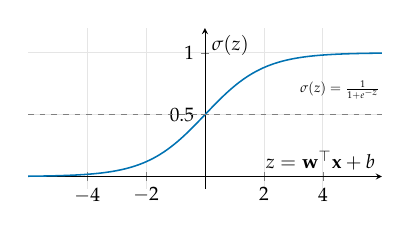
\begin{tikzpicture}[scale=0.7]
    \begin{axis}[
        xlabel={$z = \vw^\top \vx + b$}, ylabel={$\sigma(z)$},
        xmin=-6, xmax=6, ymin=-0.1, ymax=1.2,
        width=8cm, height=4.5cm,
        axis lines=middle,
        ytick={0, 0.5, 1},
        xtick={-4, -2, 0, 2, 4},
        grid=major, grid style={gray!20}
    ]
    \addplot[thick, blue, samples=100, domain=-6:6] {1/(1+exp(-x))};
    \draw[dashed, gray] (axis cs:-6,0.5) -- (axis cs:6,0.5);
    \node[right, font=\scriptsize] at (axis cs:3, 0.7) {$\sigma(z) = \frac{1}{1+e^{-z}}$};
    \end{axis}
\end{tikzpicture}
\end{center}

\vspace{2pt}
\textbf{Properties:}
$\sigma(0) = 0.5$, \quad $\lim_{z\to\infty}\sigma(z) = 1$, \quad $\lim_{z\to-\infty}\sigma(z) = 0$, \quad $\sigma'(z) = \sigma(z)(1-\sigma(z))$.
\end{frame}

% ---- Cross-Entropy ----
\begin{frame}
\frametitle{Binary Cross-Entropy Loss}

For classification, MSE is not ideal. Instead, we use the \textbf{binary cross-entropy} loss:

\begin{tikzpicture}
\node [mybox] (box){%
    \begin{minipage}{0.93\textwidth}
    \[
        \mathcal{L}(\vw, b) = -\frac{1}{N}\sum_{i=1}^{N}\Big[ y_i \log \hat{y}_i + (1 - y_i)\log(1 - \hat{y}_i) \Big]
    \]
    where $\hat{y}_i = \sigma(\vw^\top \vx_i + b)$ is the predicted probability.
    \end{minipage}
};
\node[fancytitle, right=10pt] at (box.north west) {Binary Cross-Entropy (BCE)};
\end{tikzpicture}

\vspace{8pt}
\textbf{Intuition:}
\begin{wideitemize}
    \item If $y_i = 1$: loss $= -\log \hat{y}_i$ \quad $\Rightarrow$ penalizes when $\hat{y}_i \approx 0$ (confident wrong).
    \item If $y_i = 0$: loss $= -\log(1 - \hat{y}_i)$ \quad $\Rightarrow$ penalizes when $\hat{y}_i \approx 1$ (confident wrong).
\end{wideitemize}

\vspace{6pt}
\textbf{Derivation:} comes from \textbf{maximum likelihood estimation} (MLE):
\[
    \max_{\vw,b} \prod_{i=1}^N \hat{y}_i^{y_i}(1-\hat{y}_i)^{1-y_i} \quad \Leftrightarrow \quad \min_{\vw,b} \; \mathcal{L}(\vw,b)
\]
\end{frame}

% ---- Gradient Descent ----
\begin{frame}
\frametitle{Gradient Descent}

Unlike linear regression, most models \textbf{don't have closed-form solutions}. We use \textbf{iterative optimization}.

\begin{tikzpicture}
\node [mybox] (box){%
    \begin{minipage}{0.93\textwidth}
    Repeat until convergence:
    \[
        \vw \leftarrow \vw - \alpha \, \nabla_{\vw}\mathcal{L}(\vw, b) \qquad\qquad b \leftarrow b - \alpha \, \frac{\partial \mathcal{L}}{\partial b}
    \]
    where $\alpha > 0$ is the \textbf{learning rate}.
    \end{minipage}
};
\node[fancytitle, right=10pt] at (box.north west) {Gradient Descent Update Rule};
\end{tikzpicture}

\begin{center}
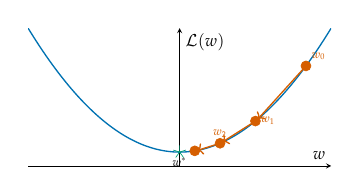
\begin{tikzpicture}[scale=0.6]
    \begin{axis}[
        xlabel={$w$}, ylabel={$\mathcal{L}(w)$},
        xmin=-3, xmax=3, ymin=0, ymax=5,
        width=8cm, height=4.5cm,
        axis lines=middle, ticks=none
    ]
    \addplot[thick, blue, domain=-3:3, samples=100] {0.5*x^2 + 0.5};

    \addplot[only marks, mark=*, mark size=3pt, red] coordinates {(2.5, 3.625) (1.5, 1.625) (0.8, 0.82) (0.3, 0.545)};

    \draw[->, thick, red] (axis cs:2.5, 3.625) -- (axis cs:1.55, 1.7);
    \draw[->, thick, red] (axis cs:1.5, 1.625) -- (axis cs:0.85, 0.87);
    \draw[->, thick, red] (axis cs:0.8, 0.82) -- (axis cs:0.35, 0.56);

    \node[above right, red, font=\scriptsize] at (axis cs:2.5, 3.625) {$w_0$};
    \node[right, red, font=\scriptsize] at (axis cs:1.5, 1.625) {$w_1$};
    \node[above, red, font=\scriptsize] at (axis cs:0.8, 0.82) {$w_2$};

    \node[below, font=\scriptsize] at (axis cs:0, 0.5) {$w^*$};
    \addplot[only marks, mark=star, mark size=4pt, green] coordinates {(0, 0.5)};
    \end{axis}
\end{tikzpicture}
\end{center}

\vspace{2pt}
\textbf{Intuition:} move in the direction of steepest descent, with step size $\alpha$.
\end{frame}

% ---- Gradient Derivation ----
\begin{frame}
\frametitle{Gradient Derivation: Linear Regression Example}

Let $f(x) = wx + b$ with a single input ($d=1$). Loss for one sample:
\[
    \ell = (y - wx - b)^2
\]

\textbf{Computing the gradients:}
\begin{align*}
    \frac{\partial \ell}{\partial w} &= \frac{\partial}{\partial w}(y - wx - b)^2 = 2(y - wx - b) \cdot (-x) = \textcolor{red}{-2x(y - wx - b)} \\[6pt]
    \frac{\partial \ell}{\partial b} &= \frac{\partial}{\partial b}(y - wx - b)^2 = 2(y - wx - b) \cdot (-1) = \textcolor{red}{-2(y - wx - b)}
\end{align*}

\textbf{For the full dataset} (average over $N$ samples):
\[
    \frac{\partial \mathcal{L}}{\partial w} = -\frac{2}{N}\sum_{i=1}^{N} x_i(y_i - wx_i - b) \qquad
    \frac{\partial \mathcal{L}}{\partial b} = -\frac{2}{N}\sum_{i=1}^{N} (y_i - wx_i - b)
\]

\textbf{Update:}
\[
    w \leftarrow w + \frac{2\alpha}{N}\sum_{i=1}^{N} x_i(y_i - wx_i - b) \qquad
    b \leftarrow b + \frac{2\alpha}{N}\sum_{i=1}^{N} (y_i - wx_i - b)
\]
\end{frame}

% ---- Learning Rate ----
\begin{frame}
\frametitle{The Learning Rate $\alpha$}

\begin{columns}
\begin{column}{0.48\textwidth}
\centering
\textcolor{blue}{\textbf{Too small: slow convergence}}

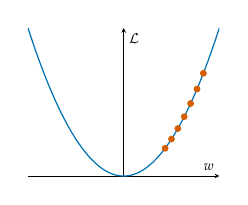
\begin{tikzpicture}[scale=0.55]
    \begin{axis}[
        width=6cm, height=5cm, axis lines=middle, ticks=none,
        xlabel={\small $w$}, ylabel={\small $\mathcal{L}$}
    ]
    \addplot[thick, blue, domain=-3:3, samples=50] {0.5*x^2 + 0.5};
    \addplot[only marks, mark=*, mark size=2pt, red] coordinates {
        (2.5, 3.625) (2.3, 3.145) (2.1, 2.705) (1.9, 2.305) (1.7, 1.945)
        (1.5, 1.625) (1.3, 1.345)
    };
    \end{axis}
\end{tikzpicture}
\end{column}

\begin{column}{0.48\textwidth}
\centering
\textcolor{red}{\textbf{Too large: divergence}}

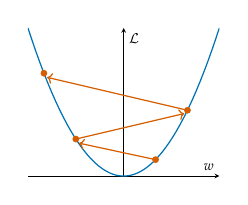
\begin{tikzpicture}[scale=0.55]
    \begin{axis}[
        width=6cm, height=5cm, axis lines=middle, ticks=none,
        xlabel={\small $w$}, ylabel={\small $\mathcal{L}$}
    ]
    \addplot[thick, blue, domain=-3:3, samples=50] {0.5*x^2 + 0.5};
    \addplot[only marks, mark=*, mark size=2pt, red] coordinates {
        (1, 1) (-1.5, 1.625) (2, 2.5) (-2.5, 3.625)
    };
    \draw[->, red, thick] (axis cs:1, 1) -- (axis cs:-1.4, 1.5);
    \draw[->, red, thick] (axis cs:-1.5, 1.625) -- (axis cs:1.9, 2.4);
    \draw[->, red, thick] (axis cs:2, 2.5) -- (axis cs:-2.4, 3.5);
    \end{axis}
\end{tikzpicture}
\end{column}
\end{columns}

\vspace{8pt}
\begin{center}
\begin{tabular}{ll}
    \toprule
    \textbf{$\alpha$ too small} & Converges, but very slowly \\
    \textbf{$\alpha$ too large} & Overshoots, may diverge \\
    \textbf{$\alpha$ just right} & Converges efficiently \\
    \bottomrule
\end{tabular}
\end{center}

\vspace{4pt}
{\small Typical starting values: $\alpha \in \{0.001, 0.01, 0.1\}$. We'll learn better strategies in Lecture 3.}
\end{frame}

% ---- Limitation ----
\begin{frame}
\frametitle{The Limitation of Linear Models}

Linear models can only produce \textbf{linear decision boundaries}.

\begin{center}
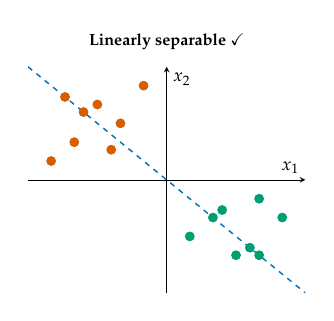
\begin{tikzpicture}[scale=0.65]
    \begin{axis}[
        xlabel={$x_1$}, ylabel={$x_2$},
        xmin=-3, xmax=3, ymin=-3, ymax=3,
        width=7cm, height=6cm,
        axis lines=middle, ticks=none,
        title={\small\textbf{Linearly separable} $\checkmark$}
    ]
    \addplot[only marks, mark=*, mark size=2.5pt, red] coordinates {
        (-2,1) (-1.5,2) (-2.5,0.5) (-1,1.5) (-0.5,2.5) (-1.8,1.8) (-2.2,2.2) (-1.2,0.8)
    };
    \addplot[only marks, mark=*, mark size=2.5pt, green] coordinates {
        (1,-1) (1.5,-2) (2,-0.5) (0.5,-1.5) (2.5,-1) (1.8,-1.8) (1.2,-0.8) (2,-2)
    };
    \addplot[thick, blue, dashed, domain=-3:3] {-x};
    \end{axis}
\end{tikzpicture}
\hspace{1cm}
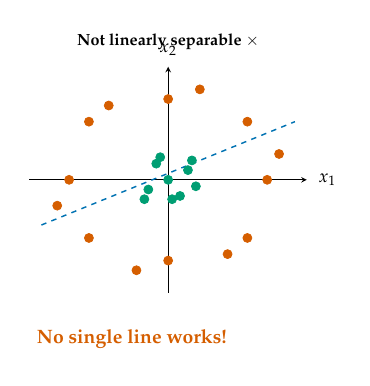
\begin{tikzpicture}[scale=0.65]
    \begin{axis}[
        xlabel={$x_1$}, ylabel={$x_2$},
        xmin=-3.5, xmax=3.5, ymin=-3.5, ymax=3.5,
        width=7cm, height=6cm,
        axis lines=middle, ticks=none,
        title={\small\textbf{Not linearly separable} $\times$},
        xlabel style={anchor=west, at={(axis description cs:1.02,0.5)}},
        ylabel style={anchor=south, at={(axis description cs:0.5,1.02)}}
    ]
    \addplot[only marks, mark=*, mark size=2.5pt, red] coordinates {
        (2.5,0) (-2.5,0) (0,2.5) (0,-2.5) (2,1.8) (-2,1.8) (2,-1.8) (-2,-1.8)
        (2.8,0.8) (-2.8,-0.8) (0.8,2.8) (-0.8,-2.8) (1.5,-2.3) (-1.5,2.3)
    };
    \addplot[only marks, mark=*, mark size=2.5pt, green] coordinates {
        (0,0) (0.5,0.3) (-0.3,0.5) (0.3,-0.5) (-0.5,-0.3) (0.7,-0.2) (-0.2,0.7) (0.1,-0.6) (-0.6,-0.6) (0.6,0.6)
    };
    \addplot[thick, blue, dashed, domain=-3.2:3.2] {0.5*x + 0.2};
    \end{axis}
    \node[font=\scriptsize\bfseries, text=red] at (2.0, -0.9) {No single line works!};
\end{tikzpicture}
\end{center}

\vspace{4pt}
\begin{center}
\textcolor{red}{We need \textbf{non-linear} models. This is where neural networks come in.}
\end{center}
\end{frame}


% ============================================================
\section{The Perceptron}
% ============================================================

\begin{transitionframe}
\begin{center}
{\Huge \textbf{The Perceptron}}
\end{center}
\end{transitionframe}

% ---- Biological Neuron ----
\begin{frame}
\frametitle{Biological Inspiration}

\begin{columns}[T]
\begin{column}{0.45\textwidth}
\textbf{Biological neuron:}
\begin{wideitemize}
    \item Receives input signals from \textbf{dendrites}.
    \item Processes them in the \textbf{cell body}.
    \item If total signal exceeds a threshold, \textbf{fires} through the \textbf{axon}.
    \item Connections have different \textbf{strengths} (synaptic weights).
\end{wideitemize}

\vspace{6pt}
{\small McCulloch \& Pitts (1943) proposed the first mathematical model of a neuron.}
\end{column}

\begin{column}{0.52\textwidth}
\begin{center}
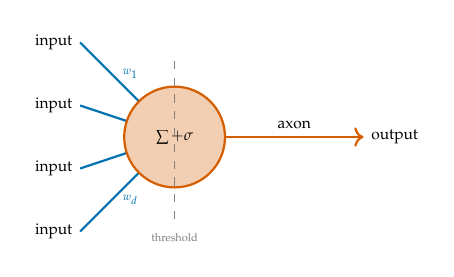
\begin{tikzpicture}[scale=0.8, every node/.style={scale=0.8}]
    \foreach \y in {-1.5, -0.5, 0.5, 1.5} {
        \draw[thick, blue] (-3, \y) -- (-1.5, 0);
        \node[left, font=\scriptsize] at (-3, \y) {input};
    }

    \draw[fill=red!30, draw=red, thick] (-1.5,0) circle (0.8cm);
    \node[font=\scriptsize\bfseries] at (-1.5, 0) {$\sum + \sigma$};

    \draw[thick, red, ->] (-0.7, 0) -- (1.5, 0);
    \node[above, font=\scriptsize] at (0.4, 0) {axon};

    \node[right, font=\scriptsize] at (1.5, 0) {output};

    \node[above, font=\tiny, blue] at (-2.2, 0.8) {$w_1$};
    \node[below, font=\tiny, blue] at (-2.2, -0.8) {$w_d$};

    \draw[dashed, gray] (-1.5, -1.3) -- (-1.5, 1.3);
    \node[below, font=\tiny, gray] at (-1.5, -1.4) {threshold};
\end{tikzpicture}
\end{center}

\vspace{6pt}
\begin{center}
\small The analogy is \textbf{loose}. Real neurons are far more complex. But the abstraction is powerful.
\end{center}
\end{column}
\end{columns}
\end{frame}

% ---- Artificial Neuron ----
\begin{frame}
\frametitle{The Artificial Neuron (Perceptron)}

\begin{center}
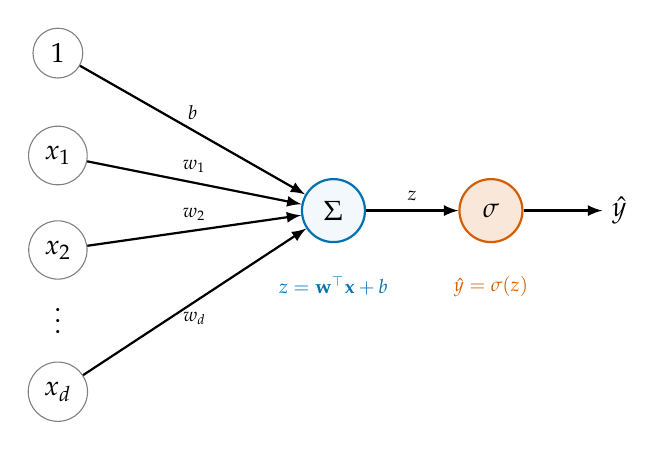
\begin{tikzpicture}[
    node distance=1.2cm and 1.8cm,
    neuron/.style={circle, draw=blue, thick, minimum size=0.8cm, fill=blue!5},
    input/.style={circle, draw=gray, minimum size=0.6cm},
    >=latex
]
    \node[input] (b) at (0, 2.5) {$1$};
    \node[input] (x1) at (0, 1.2) {$x_1$};
    \node[input] (x2) at (0, 0) {$x_2$};
    \node at (0, -0.8) {$\vdots$};
    \node[input] (xd) at (0, -1.8) {$x_d$};

    \node[neuron] (sum) at (3.5, 0.5) {$\Sigma$};

    \node[neuron, fill=red!15, draw=red] (act) at (5.5, 0.5) {$\sigma$};

    \node[right=1cm of act, font=\bfseries] (out) {$\hat{y}$};

    \draw[->, thick] (b) -- node[above, font=\scriptsize] {$b$} (sum);
    \draw[->, thick] (x1) -- node[above, font=\scriptsize] {$w_1$} (sum);
    \draw[->, thick] (x2) -- node[above, font=\scriptsize] {$w_2$} (sum);
    \draw[->, thick] (xd) -- node[below, font=\scriptsize] {$w_d$} (sum);

    \draw[->, thick] (sum) -- node[above, font=\scriptsize] {$z$} (act);

    \draw[->, thick] (act) -- (out);

    \node[below=0.3cm of sum, font=\scriptsize, blue] {$z = \vw^\top\vx + b$};
    \node[below=0.3cm of act, font=\scriptsize, red] {$\hat{y} = \sigma(z)$};
\end{tikzpicture}
\end{center}

\begin{tikzpicture}
\node [mybox] (box){%
    \begin{minipage}{0.93\textwidth}
    \[
        \hat{y} = \sigma\!\left(\sum_{j=1}^{d} w_j x_j + b\right) = \sigma(\vw^\top \vx + b)
    \]
    \begin{itemize}
        \item $\vx \in \R^d$: input features. \quad $\vw \in \R^d$: learnable weights. \quad $b \in \R$: bias.
        \item $\sigma(\cdot)$: \textbf{activation function} (introduces non-linearity).
    \end{itemize}
    \end{minipage}
};
\node[fancytitle, right=10pt] at (box.north west) {The Perceptron};
\end{tikzpicture}
\end{frame}

% ---- Activation Functions ----
\begin{frame}
\frametitle{Activation Functions}

The activation function $\sigma$ introduces \textbf{non-linearity} into the model.

\vspace{4pt}
\begin{center}
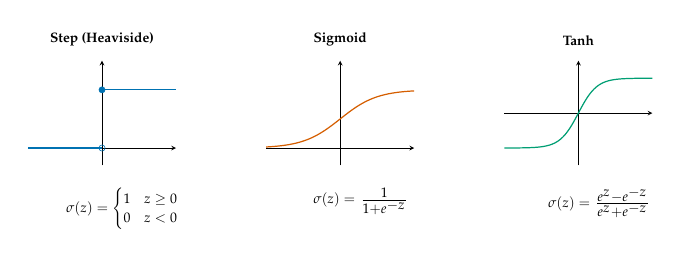
\begin{tikzpicture}[scale=0.55]
    \begin{scope}[shift={(0,0)}]
        \begin{axis}[
            title={\small\textbf{Step (Heaviside)}},
            width=5cm, height=4cm,
            xmin=-4, xmax=4, ymin=-0.3, ymax=1.5,
            axis lines=middle, ticks=none
        ]
        \addplot[thick, blue, domain=-4:0] {0};
        \addplot[thick, blue, domain=0:4] {1};
        \addplot[only marks, mark=*, mark size=2pt, blue] coordinates {(0,1)};
        \addplot[only marks, mark=o, mark size=2pt, blue] coordinates {(0,0)};
        \end{axis}
        \node[below, font=\tiny] at (2.2, -0.3) {$\sigma(z) = \begin{cases}1 & z \geq 0 \\ 0 & z < 0\end{cases}$};
    \end{scope}

    \begin{scope}[shift={(5.5,0)}]
        \begin{axis}[
            title={\small\textbf{Sigmoid}},
            width=5cm, height=4cm,
            xmin=-4, xmax=4, ymin=-0.3, ymax=1.5,
            axis lines=middle, ticks=none
        ]
        \addplot[thick, red, domain=-4:4, samples=100] {1/(1+exp(-x))};
        \end{axis}
        \node[below, font=\tiny] at (2.2, -0.3) {$\sigma(z) = \frac{1}{1+e^{-z}}$};
    \end{scope}

    \begin{scope}[shift={(11,0)}]
        \begin{axis}[
            title={\small\textbf{Tanh}},
            width=5cm, height=4cm,
            xmin=-4, xmax=4, ymin=-1.5, ymax=1.5,
            axis lines=middle, ticks=none
        ]
        \addplot[thick, green, domain=-4:4, samples=100] {tanh(x)};
        \end{axis}
        \node[below, font=\tiny] at (2.2, -0.3) {$\sigma(z) = \frac{e^z - e^{-z}}{e^z + e^{-z}}$};
    \end{scope}
\end{tikzpicture}

\vspace{8pt}
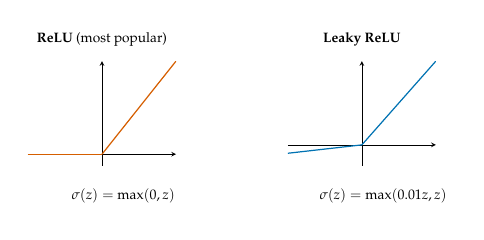
\begin{tikzpicture}[scale=0.55]
    \begin{scope}[shift={(2.5,0)}]
        \begin{axis}[
            title={\small\textbf{ReLU} (most popular)},
            width=5cm, height=4cm,
            xmin=-4, xmax=4, ymin=-0.5, ymax=4,
            axis lines=middle, ticks=none
        ]
        \addplot[thick, red, domain=-4:0] {0};
        \addplot[thick, red, domain=0:4] {x};
        \end{axis}
        \node[below, font=\tiny] at (2.2, -0.3) {$\sigma(z) = \max(0, z)$};
    \end{scope}

    \begin{scope}[shift={(8.5,0)}]
        \begin{axis}[
            title={\small\textbf{Leaky ReLU}},
            width=5cm, height=4cm,
            xmin=-4, xmax=4, ymin=-1, ymax=4,
            axis lines=middle, ticks=none
        ]
        \addplot[thick, blue, domain=-4:0] {0.1*x};
        \addplot[thick, blue, domain=0:4] {x};
        \end{axis}
        \node[below, font=\tiny] at (2.2, -0.3) {$\sigma(z) = \max(0.01z, z)$};
    \end{scope}
\end{tikzpicture}
\end{center}
\end{frame}

% ---- Why Non-linearity ----
\begin{frame}
\frametitle{Why Do We Need Non-linearity?}

\textcolor{red}{\textbf{Critical Insight:}} Without activation functions, a multi-layer network collapses to a \textbf{single linear transformation}.

\vspace{6pt}
\textbf{Proof:} Consider two linear layers (no activation):
\begin{align*}
    \vh^{(1)} &= \vW^{(1)}\vx + \vb^{(1)} \\
    \hat{\vy} &= \vW^{(2)}\vh^{(1)} + \vb^{(2)} = \vW^{(2)}(\vW^{(1)}\vx + \vb^{(1)}) + \vb^{(2)}
\end{align*}

\[
    = \underbrace{\vW^{(2)}\vW^{(1)}}_{\vW'}\vx + \underbrace{\vW^{(2)}\vb^{(1)} + \vb^{(2)}}_{\vb'} = \vW'\vx + \vb'
\]

\vspace{4pt}
This is just \textbf{another linear model}! The depth is useless.

\vspace{8pt}
\begin{center}
\fbox{\textbf{Non-linear activations are what make depth meaningful.}}
\end{center}

\vspace{6pt}
With activations: $\hat{\vy} = \vW^{(2)}\sigma(\vW^{(1)}\vx + \vb^{(1)}) + \vb^{(2)}$ \quad $\Rightarrow$ \textcolor{red}{genuinely non-linear}.
\end{frame}

% ---- XOR Problem ----
\begin{frame}
\frametitle{The XOR Problem: Why One Layer Is Not Enough}

\textbf{Boolean operations with a single perceptron:}

\begin{center}
\begin{tikzpicture}[scale=0.6]
    \begin{scope}[shift={(0,0)}]
        \begin{axis}[
            title={\small\textbf{AND} $\checkmark$},
            width=5cm, height=5cm,
            xmin=-0.6, xmax=1.6, ymin=-0.6, ymax=1.6,
            axis lines=middle, ticks=none,
            xtick={0,1}, ytick={0,1},
            xlabel={\tiny $x_1$}, ylabel={\tiny $x_2$},
            xlabel style={anchor=west, at={(axis description cs:1.02,0.25)}},
            ylabel style={anchor=south, at={(axis description cs:0.25,1.02)}}
        ]
        \addplot[only marks, mark=*, mark size=4pt, red] coordinates {(0,0) (0,1) (1,0)};
        \addplot[only marks, mark=*, mark size=4pt, green] coordinates {(1,1)};
        \addplot[thick, blue, dashed, domain=0.2:1.3] {-x + 1.5};
        \end{axis}
    \end{scope}

    \begin{scope}[shift={(6,0)}]
        \begin{axis}[
            title={\small\textbf{OR} $\checkmark$},
            width=5cm, height=5cm,
            xmin=-0.6, xmax=1.6, ymin=-0.6, ymax=1.6,
            axis lines=middle, ticks=none,
            xtick={0,1}, ytick={0,1},
            xlabel={\tiny $x_1$}, ylabel={\tiny $x_2$},
            xlabel style={anchor=west, at={(axis description cs:1.02,0.25)}},
            ylabel style={anchor=south, at={(axis description cs:0.25,1.02)}}
        ]
        \addplot[only marks, mark=*, mark size=4pt, red] coordinates {(0,0)};
        \addplot[only marks, mark=*, mark size=4pt, green] coordinates {(0,1) (1,0) (1,1)};
        \addplot[thick, blue, dashed, domain=-0.3:0.8] {-x + 0.5};
        \end{axis}
    \end{scope}

    \begin{scope}[shift={(12,0)}]
        \begin{axis}[
            title={\small\textbf{XOR} $\times$},
            width=5cm, height=5cm,
            xmin=-0.6, xmax=1.6, ymin=-0.6, ymax=1.6,
            axis lines=middle, ticks=none,
            xtick={0,1}, ytick={0,1},
            xlabel={\tiny $x_1$}, ylabel={\tiny $x_2$},
            xlabel style={anchor=west, at={(axis description cs:1.02,0.25)}},
            ylabel style={anchor=south, at={(axis description cs:0.25,1.02)}}
        ]
        \addplot[only marks, mark=*, mark size=4pt, red] coordinates {(0,0) (1,1)};
        \addplot[only marks, mark=*, mark size=4pt, green] coordinates {(0,1) (1,0)};
        \end{axis}
        \node[font=\scriptsize\bfseries, text=red] at (1.25, -2.5) {No single line!};
    \end{scope}
\end{tikzpicture}
\end{center}

\vspace{4pt}
\begin{wideitemize}
    \item AND and OR are \textbf{linearly separable} --- a single perceptron can learn them.
    \item XOR is \textbf{not linearly separable} --- requires composing multiple linear boundaries.
    \item Shown by \textbf{Minsky \& Papert (1969)} and caused the first ``AI winter''.
\end{wideitemize}
\end{frame}

% ---- Solving XOR (Part 1) ----
\begin{frame}
\frametitle{Solving XOR with Two Layers}

\textbf{Key insight:} XOR $= $ AND(OR($x_1, x_2$), NAND($x_1, x_2$))

\vspace{8pt}
\begin{center}
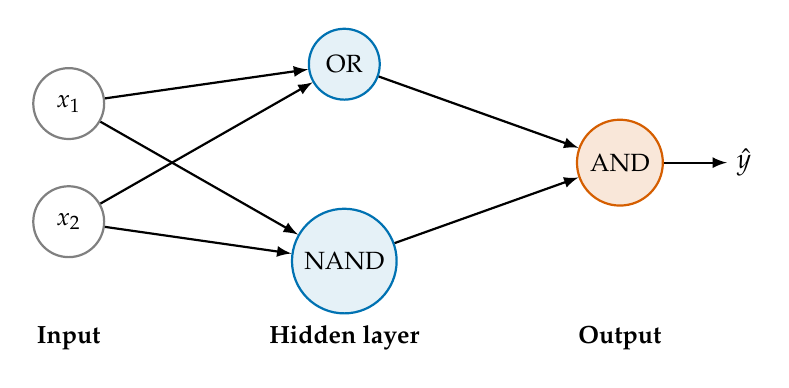
\begin{tikzpicture}[
    neuron/.style={circle, draw, thick, minimum size=0.9cm, font=\small},
    >=latex,
    scale=1
]
    \node[neuron, draw=gray] (x1) at (0, 1.5) {$x_1$};
    \node[neuron, draw=gray] (x2) at (0, 0) {$x_2$};

    \node[neuron, draw=blue, fill=blue!10] (h1) at (3.5, 2) {OR};
    \node[neuron, draw=blue, fill=blue!10] (h2) at (3.5, -0.5) {NAND};

    \node[neuron, draw=red, fill=red!15] (out) at (7, 0.75) {AND};

    \node[right=0.8cm of out, font=\bfseries] (y) {$\hat{y}$};

    \draw[->, thick] (x1) -- (h1);
    \draw[->, thick] (x1) -- (h2);
    \draw[->, thick] (x2) -- (h1);
    \draw[->, thick] (x2) -- (h2);
    \draw[->, thick] (h1) -- (out);
    \draw[->, thick] (h2) -- (out);
    \draw[->, thick] (out) -- (y);

    \node[below, font=\small\bfseries] at (0, -1.2) {Input};
    \node[below, font=\small\bfseries] at (3.5, -1.2) {Hidden layer};
    \node[below, font=\small\bfseries] at (7, -1.2) {Output};
\end{tikzpicture}
\end{center}

\vspace{8pt}
\begin{center}
\textcolor{red}{Adding one hidden layer solves the problem! This is the power of depth.}
\end{center}
\end{frame}

% ---- Solving XOR (Part 2 - truth table) ----
\begin{frame}
\frametitle{XOR: Truth Table Verification}

The hidden layer computes OR and NAND; the output layer applies AND.

\vspace{10pt}
\begin{center}
\renewcommand{\arraystretch}{1.4}
\begin{tabular}{cc|c|c|c}
    \toprule
    $x_1$ & $x_2$ & OR$(x_1,x_2)$ & NAND$(x_1,x_2)$ & AND(OR, NAND) = \textbf{XOR} \\
    \midrule
    0 & 0 & 0 & 1 & \textbf{0} \\
    0 & 1 & 1 & 1 & \textbf{1} \\
    1 & 0 & 1 & 1 & \textbf{1} \\
    1 & 1 & 1 & 0 & \textbf{0} \\
    \bottomrule
\end{tabular}
\end{center}

\vspace{10pt}
\begin{wideitemize}
    \item The hidden layer \textbf{transforms} the input into a new representation.
    \item In the new representation, the two classes \textbf{are} linearly separable.
    \item This is the essence of deep learning: \textcolor{red}{learn useful representations, then classify}.
\end{wideitemize}
\end{frame}

% ---- XOR Math ----
\begin{frame}
\frametitle{XOR: The Explicit Computation}

Using step activation $\sigma(z) = \mathbbm{1}[z > 0]$:

\vspace{4pt}
\textbf{Hidden layer:}
\begin{align*}
    h_1 &= \sigma(x_1 + x_2 - 0.5) && \text{(OR: fires if $x_1 + x_2 > 0.5$)} \\
    h_2 &= \sigma(-x_1 - x_2 + 1.5) && \text{(NAND: fires if $x_1 + x_2 < 1.5$)}
\end{align*}

\textbf{Output layer:}
\[
    \hat{y} = \sigma(h_1 + h_2 - 1.5) \qquad \text{(AND: fires if $h_1 + h_2 > 1.5$)}
\]

\vspace{4pt}
\textbf{In matrix form:}
\[
    \vW^{(1)} = \begin{pmatrix} 1 & 1 \\ -1 & -1 \end{pmatrix}, \quad
    \vb^{(1)} = \begin{pmatrix} -0.5 \\ 1.5 \end{pmatrix}, \quad
    \vW^{(2)} = \begin{pmatrix} 1 & 1 \end{pmatrix}, \quad
    b^{(2)} = -1.5
\]

\vspace{4pt}
\textbf{Verify for $(x_1, x_2) = (1, 0)$:}
\[
    \vh = \sigma\!\left(\begin{pmatrix}1 & 1 \\ -1 & -1\end{pmatrix}\begin{pmatrix}1\\0\end{pmatrix} + \begin{pmatrix}-0.5\\1.5\end{pmatrix}\right) = \sigma\!\begin{pmatrix}0.5\\0.5\end{pmatrix} = \begin{pmatrix}1\\1\end{pmatrix}
\]
\[
    \hat{y} = \sigma(1 + 1 - 1.5) = \sigma(0.5) = 1 \quad \checkmark
\]
\end{frame}


% ============================================================
\section{From Perceptrons to Deep Networks}
% ============================================================

\begin{transitionframe}
\begin{center}
{\Huge \textbf{From Perceptrons to Deep Neural Networks}}
\end{center}
\end{transitionframe}

% ---- One Neuron to Layer ----
\begin{frame}
\frametitle{From One Neuron to a Layer}

\textbf{One neuron:} computes a single output feature
\[
    h_j = \sigma\!\left(\sum_{k=1}^{d} w_{jk}\, x_k + b_j\right) = \sigma(\vw_j^\top \vx + b_j)
\]

\textbf{A layer of $m$ neurons:} computes $m$ output features simultaneously
\[
    \vh = \sigma(\vW\vx + \vb) = \begin{pmatrix} \sigma(\vw_1^\top\vx + b_1) \\ \sigma(\vw_2^\top\vx + b_2) \\ \vdots \\ \sigma(\vw_m^\top\vx + b_m) \end{pmatrix} \in \R^m
\]

where $\vW \in \R^{m \times d}$ and $\vb \in \R^m$.

\vspace{6pt}
\begin{center}
\textcolor{red}{Each neuron in the layer learns a \textbf{different linear boundary}; the activation function makes each one non-linear.}
\end{center}
\end{frame}

% ---- Layer Diagram ----
\begin{frame}
\frametitle{A Fully Connected Layer}

\begin{center}
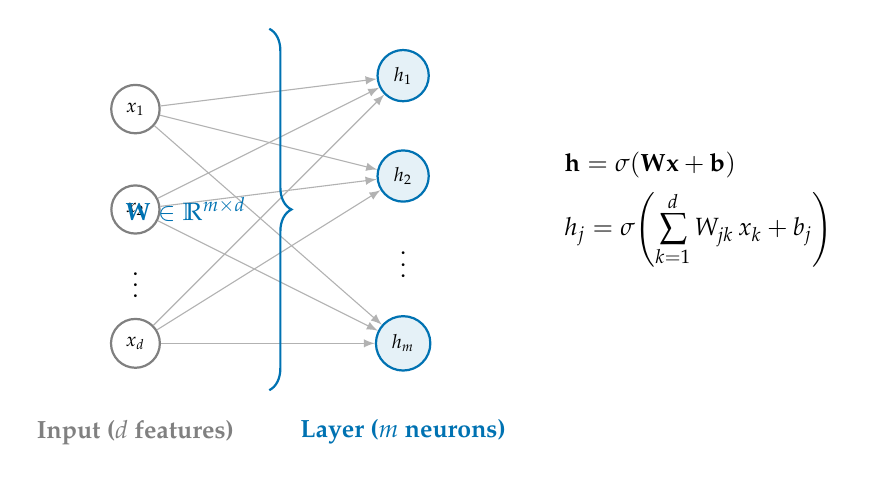
\begin{tikzpicture}[
    neuron/.style={circle, draw, thick, minimum size=0.6cm, font=\scriptsize},
    >=latex,
    scale=0.85
]
    \node[neuron, draw=gray] (i1) at (0, 3) {$x_1$};
    \node[neuron, draw=gray] (i2) at (0, 1.5) {$x_2$};
    \node at (0, 0.5) {\small$\vdots$};
    \node[neuron, draw=gray] (id) at (0, -0.5) {$x_d$};

    \node[neuron, fill=blue!10, draw=blue] (h1) at (4, 3.5) {$h_1$};
    \node[neuron, fill=blue!10, draw=blue] (h2) at (4, 2) {$h_2$};
    \node at (4, 0.8) {\small$\vdots$};
    \node[neuron, fill=blue!10, draw=blue] (hm) at (4, -0.5) {$h_m$};

    \foreach \i in {i1, i2, id} {
        \foreach \h in {h1, h2, hm} {
            \draw[->, thin, gray!60] (\i) -- (\h);
        }
    }

    \draw[decorate, decoration={brace, amplitude=8pt}, thick, blue]
        (2, 4.2) -- (2, -1.2);
    \node[blue, font=\small\bfseries, left] at (1.8, 1.5) {$\vW \in \R^{m \times d}$};

    \node[below, font=\small\bfseries, gray] at (0, -1.5) {Input ($d$ features)};
    \node[below, font=\small\bfseries, blue] at (4, -1.5) {Layer ($m$ neurons)};

    \node[right=1.5cm of hm, font=\small, align=left] at (4.5, 1.5) {
        $\vh = \sigma(\vW\vx + \vb)$\\[4pt]
        $h_j = \sigma\!\left(\displaystyle\sum_{k=1}^{d} W_{jk}\, x_k + b_j\right)$
    };
\end{tikzpicture}
\end{center}

\vspace{4pt}
\textbf{Every input is connected to every neuron:} this is called a \textbf{fully connected} (or \textbf{dense}) layer.

Parameters: $m \times d$ weights + $m$ biases $= m(d+1)$ total.
\end{frame}

% ---- Stacking Layers ----
\begin{frame}
\frametitle{Stacking Layers: The Deep Neural Network}

\textbf{A feedforward neural network} is a composition of layers:

\begin{tikzpicture}
\node [mybox] (box){%
    \begin{minipage}{0.93\textwidth}
    \begin{align*}
        \vh^{(0)} &= \vx && \text{(input)} \\
        \vh^{(1)} &= \sigma(\vW^{(1)}\vh^{(0)} + \vb^{(1)}) && \text{(hidden layer 1)} \\
        \vh^{(2)} &= \sigma(\vW^{(2)}\vh^{(1)} + \vb^{(2)}) && \text{(hidden layer 2)} \\
        &\;\;\vdots \\
        \vh^{(L-1)} &= \sigma(\vW^{(L-1)}\vh^{(L-2)} + \vb^{(L-1)}) && \text{(hidden layer $L-1$)} \\
        \hat{\vy} &= \vW^{(L)}\vh^{(L-1)} + \vb^{(L)} && \text{(output layer)}
    \end{align*}
    \end{minipage}
};
\node[fancytitle, right=10pt] at (box.north west) {Feedforward Neural Network with $L$ layers};
\end{tikzpicture}

\vspace{6pt}
\textbf{Terminology:}
\begin{wideitemize}
    \item \textbf{Depth:} number of layers $L$ (``deep'' $= L \geq 2$ hidden layers).
    \item \textbf{Width:} number of neurons per layer ($m^{(l)}$).
    \item \textbf{Parameters:} $\theta = \{\vW^{(1)}, \vb^{(1)}, \ldots, \vW^{(L)}, \vb^{(L)}\}$.
\end{wideitemize}
\end{frame}

% ---- Network Diagram ----
\begin{frame}
\frametitle{Deep Neural Network: Diagram}

\begin{center}
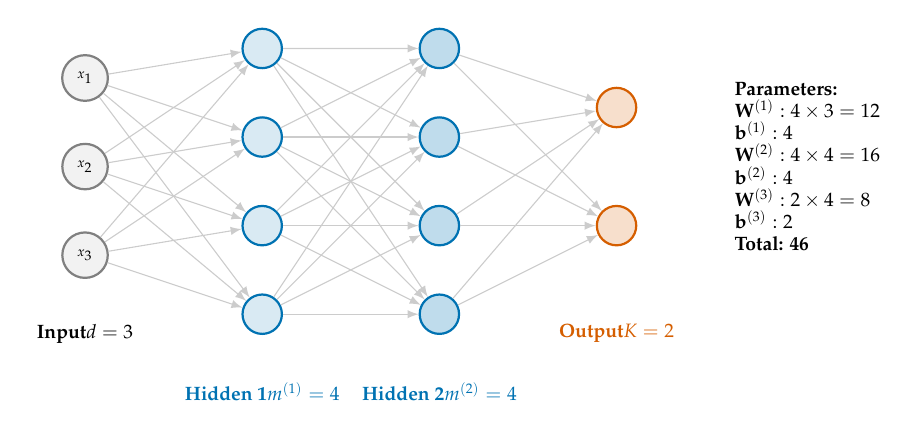
\begin{tikzpicture}[
    neuron/.style={circle, draw, thick, minimum size=0.5cm, font=\tiny},
    >=latex,
    scale=0.75
]
    \foreach \i/\y in {1/3, 2/1.5, 3/0} {
        \node[neuron, draw=gray, fill=gray!10] (i\i) at (0, \y) {$x_\i$};
    }
    \node[below, font=\scriptsize\bfseries] at (0, -1) {Input\\$d=3$};

    \foreach \i/\y in {1/3.5, 2/2, 3/0.5, 4/-1} {
        \node[neuron, fill=blue!15, draw=blue] (h1\i) at (3, \y) {};
    }
    \node[below, font=\scriptsize\bfseries, blue] at (3, -2) {Hidden 1\\$m^{(1)}=4$};

    \foreach \i/\y in {1/3.5, 2/2, 3/0.5, 4/-1} {
        \node[neuron, fill=blue!25, draw=blue] (h2\i) at (6, \y) {};
    }
    \node[below, font=\scriptsize\bfseries, blue] at (6, -2) {Hidden 2\\$m^{(2)}=4$};

    \foreach \i/\y in {1/2.5, 2/0.5} {
        \node[neuron, fill=red!20, draw=red] (o\i) at (9, \y) {};
    }
    \node[below, font=\scriptsize\bfseries, red] at (9, -1) {Output\\$K=2$};

    \foreach \i in {1,2,3} {
        \foreach \j in {1,2,3,4} {
            \draw[->, thin, gray!40] (i\i) -- (h1\j);
        }
    }

    \foreach \i in {1,2,3,4} {
        \foreach \j in {1,2,3,4} {
            \draw[->, thin, gray!40] (h1\i) -- (h2\j);
        }
    }

    \foreach \i in {1,2,3,4} {
        \foreach \j in {1,2} {
            \draw[->, thin, gray!40] (h2\i) -- (o\j);
        }
    }

    \node[right=1cm of o1, font=\scriptsize, align=left] at (9.5, 1.5) {
        \textbf{Parameters:}\\
        $\vW^{(1)}: 4 \times 3 = 12$\\
        $\vb^{(1)}: 4$\\
        $\vW^{(2)}: 4 \times 4 = 16$\\
        $\vb^{(2)}: 4$\\
        $\vW^{(3)}: 2 \times 4 = 8$\\
        $\vb^{(3)}: 2$\\
        \textbf{Total: 46}
    };
\end{tikzpicture}
\end{center}

\vspace{4pt}
\begin{center}
{\small Modern networks: GPT-4 has $\sim$1.8 \textbf{trillion} parameters. ResNet-50 has $\sim$25 million.}
\end{center}
\end{frame}

% ---- Forward Pass Example ----
\begin{frame}
\frametitle{Forward Pass: A Numerical Example}

\textbf{Network:} 2 inputs $\to$ 2 hidden (ReLU) $\to$ 1 output (linear)

\vspace{4pt}
\textbf{Given:} $\vx = \begin{pmatrix}1\\2\end{pmatrix}$, \;
$\vW^{(1)} = \begin{pmatrix}0.5 & -0.3\\0.2 & 0.8\end{pmatrix}$, \;
$\vb^{(1)} = \begin{pmatrix}0.1\\-0.1\end{pmatrix}$, \;
$\vW^{(2)} = \begin{pmatrix}0.6 & -0.4\end{pmatrix}$, \;
$b^{(2)} = 0.2$

\vspace{6pt}
\textbf{Step 1:} Compute hidden layer pre-activation
\[
    \vz^{(1)} = \vW^{(1)}\vx + \vb^{(1)} = \begin{pmatrix}0.5 & -0.3\\0.2 & 0.8\end{pmatrix}\begin{pmatrix}1\\2\end{pmatrix} + \begin{pmatrix}0.1\\-0.1\end{pmatrix} = \begin{pmatrix}-0.1\\1.7\end{pmatrix} + \begin{pmatrix}0.1\\-0.1\end{pmatrix} = \begin{pmatrix}0.0\\1.6\end{pmatrix}
\]

\textbf{Step 2:} Apply ReLU activation
\[
    \vh^{(1)} = \text{ReLU}(\vz^{(1)}) = \begin{pmatrix}\max(0, 0.0)\\\max(0, 1.6)\end{pmatrix} = \begin{pmatrix}0.0\\1.6\end{pmatrix}
\]

\textbf{Step 3:} Compute output
\[
    \hat{y} = \vW^{(2)}\vh^{(1)} + b^{(2)} = \begin{pmatrix}0.6 & -0.4\end{pmatrix}\begin{pmatrix}0.0\\1.6\end{pmatrix} + 0.2 = -0.64 + 0.2 = \textcolor{red}{-0.44}
\]
\end{frame}

% ---- Dimensions ----
\begin{frame}
\frametitle{Dimensions Cheat Sheet}

For a network with layers of widths $d = m^{(0)}, m^{(1)}, m^{(2)}, \ldots, m^{(L)}$:

\vspace{8pt}
\begin{center}
\renewcommand{\arraystretch}{1.5}
\begin{tabular}{llll}
    \toprule
    \textbf{Layer $l$} & \textbf{$\vW^{(l)}$} & \textbf{$\vb^{(l)}$} & \textbf{$\vh^{(l)}$} \\
    \midrule
    Input ($l=0$) & --- & --- & $\R^{m^{(0)}}$ \\
    Hidden $l$ & $\R^{m^{(l)} \times m^{(l-1)}}$ & $\R^{m^{(l)}}$ & $\R^{m^{(l)}}$ \\
    Output ($l=L$) & $\R^{m^{(L)} \times m^{(L-1)}}$ & $\R^{m^{(L)}}$ & $\R^{m^{(L)}}$ \\
    \bottomrule
\end{tabular}
\end{center}

\vspace{8pt}
\textbf{Total parameters:}
\[
    \sum_{l=1}^{L} \left( m^{(l)} \times m^{(l-1)} + m^{(l)} \right) = \sum_{l=1}^{L} m^{(l)}\left(m^{(l-1)} + 1\right)
\]

\vspace{4pt}
\textbf{Example:} Input $784$ $\to$ Hidden $256$ $\to$ Hidden $128$ $\to$ Output $10$
\[
    (256 \times 785) + (128 \times 257) + (10 \times 129) = 200{,}960 + 32{,}896 + 1{,}290 = \textcolor{red}{235{,}146}
\]
\end{frame}

% ---- What Does a Network Learn ----
\begin{frame}
\frametitle{What Does a Neural Network Learn?}

\textbf{Key idea:} each layer learns a \textcolor{red}{new representation} of the data.

\vspace{6pt}
\begin{center}
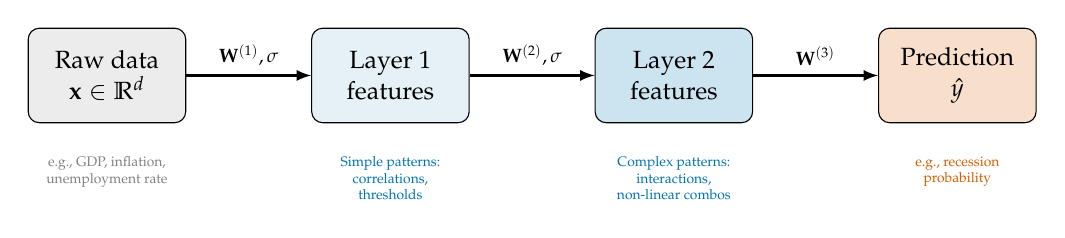
\begin{tikzpicture}[
    box/.style={rectangle, draw, rounded corners, minimum height=1.2cm, minimum width=2cm, align=center, font=\small},
    >=latex,
    scale=0.9
]
    \node[box, fill=gray!15] (raw) at (0,0) {Raw data\\$\vx \in \R^d$};
    \node[box, fill=blue!10] (h1) at (4,0) {Layer 1\\features};
    \node[box, fill=blue!20] (h2) at (8,0) {Layer 2\\features};
    \node[box, fill=red!20] (out) at (12,0) {Prediction\\$\hat{y}$};

    \draw[->, thick] (raw) -- node[above, font=\scriptsize] {$\vW^{(1)}, \sigma$} (h1);
    \draw[->, thick] (h1) -- node[above, font=\scriptsize] {$\vW^{(2)}, \sigma$} (h2);
    \draw[->, thick] (h2) -- node[above, font=\scriptsize] {$\vW^{(3)}$} (out);

    \node[below=0.3cm, font=\tiny, align=center, gray] at (raw.south) {e.g., GDP, inflation,\\unemployment rate};
    \node[below=0.3cm, font=\tiny, align=center, blue] at (h1.south) {Simple patterns:\\correlations,\\thresholds};
    \node[below=0.3cm, font=\tiny, align=center, blue] at (h2.south) {Complex patterns:\\interactions,\\non-linear combos};
    \node[below=0.3cm, font=\tiny, align=center, red] at (out.south) {e.g., recession\\probability};
\end{tikzpicture}
\end{center}

\vspace{6pt}
\textbf{For economists:} think of it as \textbf{automatic feature engineering}:
\begin{wideitemize}
    \item Instead of manually creating interaction terms ($x_1 \cdot x_2$, $x_1^2$, etc.).
    \item The network \textbf{learns} which transformations of the raw features are useful.
    \item Particularly powerful when $d$ is large (hundreds of variables).
\end{wideitemize}
\end{frame}


% ============================================================
\section{Introduction to PyTorch and Google Colab}
% ============================================================

\begin{transitionframe}
\begin{center}
{\Huge \textbf{Introduction to PyTorch \& Google Colab}}
\end{center}
\end{transitionframe}

% ---- PyTorch ----
\begin{frame}
\frametitle{Why PyTorch?}

\textbf{PyTorch} is the most widely used deep learning framework in research.

\vspace{6pt}
\begin{columns}[T]
\begin{column}{0.48\textwidth}
\textcolor{blue}{\textbf{Key features:}}
\begin{wideitemize}
    \item \textbf{Dynamic computation graphs} (define-by-run).
    \item \textbf{Automatic differentiation} (autograd).
    \item GPU acceleration (CUDA).
    \item Pythonic, intuitive API.
    \item Huge ecosystem (torchvision, torchtext, HuggingFace).
\end{wideitemize}
\end{column}

\begin{column}{0.48\textwidth}
\textcolor{blue}{\textbf{Alternatives:}}
\begin{itemize}
    \item TensorFlow / Keras (Google).
    \item JAX (Google Research).
    \item Flux.jl (Julia).
\end{itemize}

\vspace{6pt}
\textcolor{blue}{\textbf{We use PyTorch because:}}
\begin{itemize}
    \item Standard in academia.
    \item Best for learning DL concepts.
    \item HuggingFace integration (for LLMs).
\end{itemize}
\end{column}
\end{columns}
\end{frame}

% ---- Tensors ----
\begin{frame}[fragile]
\frametitle{PyTorch Tensors}

\textbf{Tensors} are the fundamental data structure --- like NumPy arrays but with GPU support.

\vspace{4pt}
\begin{lstlisting}
import torch

# Creating tensors
x = torch.tensor([1.0, 2.0, 3.0])          # 1D tensor (vector)
W = torch.randn(3, 2)                       # 2D tensor (matrix), random
b = torch.zeros(3)                          # 1D tensor of zeros

# Operations
z = W @ x + b                # Matrix-vector multiply + bias (@ = matmul)
print(z.shape)               # torch.Size([3])

# Move to GPU
device = torch.device('cuda' if torch.cuda.is_available() else 'cpu')
x_gpu = x.to(device)
W_gpu = W.to(device)
z_gpu = W_gpu @ x_gpu        # Computation happens on GPU!
\end{lstlisting}

\vspace{4pt}
\textbf{Key difference from NumPy:} tensors track computation for \textcolor{red}{automatic differentiation}.
\end{frame}

% ---- Autograd ----
\begin{frame}[fragile]
\frametitle{Automatic Differentiation (Autograd)}

PyTorch can automatically compute gradients --- the foundation of training neural networks.

\begin{lstlisting}
import torch

# Create tensors with gradient tracking
w = torch.tensor(2.0, requires_grad=True)
b = torch.tensor(1.0, requires_grad=True)
x = torch.tensor(3.0)
y_true = torch.tensor(7.0)     # target

# Forward pass: compute prediction and loss
y_pred = w * x + b             # y_pred = 2*3 + 1 = 7
loss = (y_true - y_pred) ** 2  # MSE for one sample = 0

# Backward pass: compute gradients
loss.backward()

# Gradients are now available!
print(w.grad)    # d(loss)/dw = 2*(y_true - y_pred)*(-x) = 0
print(b.grad)    # d(loss)/db = 2*(y_true - y_pred)*(-1) = 0
\end{lstlisting}

\vspace{4pt}
\textcolor{red}{\textbf{Key Insight:}} \texttt{loss.backward()} computes $\frac{\partial \mathcal{L}}{\partial w}$ and $\frac{\partial \mathcal{L}}{\partial b}$ \textbf{automatically} using the chain rule. We'll derive backpropagation in Lecture 2.
\end{frame}

% ---- Single Neuron ----
\begin{frame}[fragile]
\frametitle{Implementing a Single Neuron in PyTorch}

\begin{lstlisting}
import torch
import torch.nn as nn

# A single neuron: 2 inputs -> 1 output with sigmoid activation
class SingleNeuron(nn.Module):
    def __init__(self):
        super().__init__()
        self.linear = nn.Linear(2, 1)    # 2 inputs, 1 output
        self.sigmoid = nn.Sigmoid()

    def forward(self, x):
        z = self.linear(x)              # z = w^T x + b
        return self.sigmoid(z)          # sigma(z)

# Create the neuron and a sample input
neuron = SingleNeuron()
x = torch.tensor([[1.0, 2.0]])         # batch of 1, 2 features
y_pred = neuron(x)
print(f"Prediction: {y_pred.item():.4f}")

# Check parameters
for name, param in neuron.named_parameters():
    print(f"{name}: {param.data}")
\end{lstlisting}

\vspace{2pt}
{\small \texttt{nn.Linear(2, 1)} creates a layer with $\vW \in \R^{1\times 2}$ and $b \in \R$ (3 parameters total).}
\end{frame}

% ---- Training Loop ----
\begin{frame}[fragile]
\frametitle{The Training Loop (Preview)}

\begin{lstlisting}
# The basic training loop structure
model = SingleNeuron()
optimizer = torch.optim.SGD(model.parameters(), lr=0.01)  # SGD
criterion = nn.BCELoss()                                   # Binary CE

for epoch in range(100):
    # Forward pass
    y_pred = model(x_train)
    loss = criterion(y_pred, y_train)

    # Backward pass
    optimizer.zero_grad()    # Reset gradients to zero
    loss.backward()          # Compute gradients (backpropagation)

    # Update parameters
    optimizer.step()         # w <- w - alpha * grad

    if epoch % 10 == 0:
        print(f"Epoch {epoch}, Loss: {loss.item():.4f}")
\end{lstlisting}

\vspace{4pt}
\begin{center}
\textbf{Every DL training follows this pattern:} forward $\to$ loss $\to$ backward $\to$ update.

We'll understand \emph{exactly why} in Lecture 2 (backpropagation).
\end{center}
\end{frame}

% ---- Google Colab ----
\begin{frame}[fragile]
\frametitle{Google Colab Setup}

\begin{columns}[T]
\begin{column}{0.55\textwidth}
\textbf{Google Colab} provides free access to GPUs in the browser.

\vspace{6pt}
\textcolor{blue}{\textbf{Getting started:}}
\begin{enumerate}
    \item Go to \texttt{colab.research.google.com}.
    \item Create a new notebook.
    \item Runtime $\to$ Change runtime type $\to$ \textbf{GPU}.
    \item PyTorch is pre-installed!
\end{enumerate}

\vspace{6pt}
\textcolor{blue}{\textbf{Recommended subscriptions:}}
\begin{itemize}
    \item \textbf{Colab Pro} (\$10/mo): better GPUs, longer runtime.
    \item \textbf{Colab Pro+} (\$50/mo): even more resources.
    \item Free tier works for Lectures 1--5.
\end{itemize}
\end{column}

\begin{column}{0.42\textwidth}
\textbf{Verify GPU access:}

\vspace{4pt}
\begin{lstlisting}
import torch
print(torch.cuda.is_available())
# True
print(torch.cuda.get_device_name(0))
# Tesla T4
\end{lstlisting}

\vspace{6pt}
\textcolor{blue}{\textbf{Also recommended:}}
\begin{itemize}
    \item \textbf{Claude Code} (\$20/mo) for coding assistance.
    \item Use LLMs as a learning tool, not a replacement.
\end{itemize}
\end{column}
\end{columns}
\end{frame}


% ============================================================
\section{Summary and Next Steps}
% ============================================================

\begin{transitionframe}
\begin{center}
{\Huge \textbf{Summary \& Next Steps}}
\end{center}
\end{transitionframe}

% ---- Summary ----
\begin{frame}
\frametitle{Lecture 1 Summary}

\begin{enumerate}
    \item \textbf{Supervised learning:} given data $\{(\vx_i, y_i)\}$, find $f$ that generalizes.

    \item \textbf{Linear models} (regression/logistic) are the starting point:
    \[
        f(\vx) = \vw^\top\vx + b \qquad \text{or} \qquad p(y=1|\vx) = \sigma(\vw^\top\vx + b)
    \]

    \item \textbf{Gradient descent} iteratively minimizes the loss:
    \[
        \vw \leftarrow \vw - \alpha \nabla_{\vw}\mathcal{L}
    \]

    \item \textbf{The perceptron} = linear model + activation function. Learns AND, OR but \textcolor{red}{not XOR}.

    \item \textbf{Deep neural networks} stack layers of perceptrons:
    \[
        \vh^{(l)} = \sigma(\vW^{(l)}\vh^{(l-1)} + \vb^{(l)})
    \]

    \item \textbf{Non-linear activations} (ReLU, sigmoid) are essential --- without them, depth is useless.

    \item \textbf{PyTorch} provides tensors + autograd for implementation.
\end{enumerate}
\end{frame}

% ---- Next Lecture ----
\begin{frame}
\frametitle{Next Lecture: Backpropagation \& Gradient Descent}

\textbf{Lecture 2} (Friday, April 17):
\begin{wideitemize}
    \item How does the network actually \textbf{learn}?
    \item The \textbf{chain rule} and backpropagation algorithm.
    \item Full derivation of gradients for multi-layer networks.
    \item Loss functions in detail: MSE, cross-entropy, softmax.
    \item Gradient descent variants.
\end{wideitemize}

\vspace{10pt}
\textbf{Recommended reading:}
\begin{itemize}
    \item Goodfellow et al., \textit{Deep Learning}, Chapters 6.1--6.3.
    \item Zhang et al., \textit{Dive into Deep Learning}, Chapters 3--4 (\url{https://d2l.ai}).
\end{itemize}

\vspace{10pt}
\textbf{Homework 1} will be released after Lecture 3 (April 20).

\vspace{6pt}
\begin{center}
\Large \textcolor{blue}{\textbf{Questions?}}
\end{center}
\end{frame}

% ---- References ----
\begin{frame}
\frametitle{References}

\small
\begin{wideitemize}
    \item Goodfellow, I., Bengio, Y., \& Courville, A. (2016). \textit{Deep Learning}. MIT Press.
    \item Zhang, A., Lipton, Z. C., Li, M., \& Smola, A. J. (2023). \textit{Dive into Deep Learning}. Cambridge University Press.
    \item Rosenblatt, F. (1958). The Perceptron: A probabilistic model for information storage and organization in the brain. \textit{Psychological Review}, 65(6), 386.
    \item Minsky, M., \& Papert, S. (1969). \textit{Perceptrons}. MIT Press.
    \item Jean, N. et al. (2016). Combining Satellite Imagery and Machine Learning to Predict Poverty. \textit{Science}, 353(6301), 790--794.
    \item Gentzkow, M., Kelly, B., \& Taddy, M. (2019). Text as Data. \textit{Journal of Economic Literature}, 57(3), 535--574.
    \item Athey, S., \& Imbens, G. W. (2019). Machine Learning Methods That Economists Should Know About. \textit{Annual Review of Economics}, 11, 685--725.
    \item Hansen, S., \& McMahon, M. (2016). Shocking Language. \textit{Journal of International Economics}, 99.
\end{wideitemize}
\end{frame}

\end{document}
